\documentclass{article}
\usepackage{listings}
\usepackage{caption}
\usepackage{xcolor}
\usepackage{graphicx}
\usepackage{multirow}
\usepackage{amsmath}
\usepackage{hyperref}
\usepackage[utf8]{inputenc}

\definecolor{codegreen}{rgb}{0,0.6,0}
\definecolor{codegray}{rgb}{0.5,0.5,0.5}
\definecolor{codepurple}{rgb}{0.58,0,0.82}
\definecolor{backcolour}{rgb}{0.95,0.95,0.92}

\definecolor{page}{RGB}{43, 43, 43}

\lstdefinestyle{mystyle}{
    backgroundcolor=\color{white},   
    commentstyle=\color{codegreen},
    keywordstyle=\color{magenta},
    numberstyle=\tiny\color{codegray},
    stringstyle=\color{codepurple},
    basicstyle=\ttfamily\footnotesize,
    breakatwhitespace=false,         
    breaklines=true,                 
    captionpos=b,                    
    keepspaces=true,                 
    numbers=left,                    
    numbersep=5pt,                  
    showspaces=false,                
    showstringspaces=false,
    showtabs=false,                  
    tabsize=2
}

\lstset{style=mystyle}

\title{Algorithms: Design \& Analysis\\Project Report}
\author{Owais Bin Asad (oa05007) \and Aaron Lucas Soares (as04345) \and Bahzad Ahmed Badvi (bb05083)}
\date{5\textsuperscript{th} December 2020}

\begin{document}

\maketitle

\section{Introduction}
This project deals with the topic of Matrix multiplication, the relevance of this topic stems from the fact that matrix multiplication is a hefty operation in terms of time and is used quite often. This project aims to explore two different algorithms for matrix multiplication and analyze them, both empirically and theoretically.

\section{Repository}
The algorithm implementations, empirical analysis code, and report .tex file can be found \href{https://www.google.com}{here}.

\section{Algorithms}
\begin{itemize}
    \item Naive Method
    \item Strassen's Method
\end{itemize}

\section{Implementation}
\subsection{Naive Method}
\lstinputlisting[language=Python, caption=Naive Method]{naive.py}

\subsection{Strassen's Method}
\lstinputlisting[language=Python, caption=Strassen's Method]{strassen.py}

\section{Theoretical Comparison}
\subsection{Naive Method}
The naive implementation employs the simple method of multiplying a row of one matrix with the corresponding column of the other matrix to obtain an element of the resultant matrix.\\
Suppose we had two $n\times n$ matrices $A$ and $B$ which were being multiplied and a $n\times n$ matrix $R$ which is our resultant matrix. To obtain the $R_{1,1}$ element, we would multiply the first row of A with the first column of B. Similarly, to obtain $R_{2,3}$, we would need to multiply the second row of A with the third row of B.
\\
To carry out this simple multiplication, the naive method uses three loops each running for $n$ iterations. Therefore, this implementation has a time complexity of $O(n^3)$.


\subsection{Strassen's Method}

\subsubsection{A Divide and Conquer Approach}
Suppose we have 2 matrices with dimensions n by n. The algorithm will recursively divide each of these matrices into 4 smaller sub-matrices, each having dimensions n/2 by n/2. It then calculates 8 multiplications which take O(n) time and 4 additions which will take $O(n^2)$ time. 

\begin{figure}[h!]
    \centering
    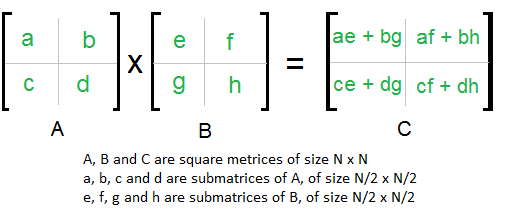
\includegraphics[scale=0.8]{dnc.png}
    \caption{Divide and Conquer Approach}
    \caption*{Source: www.geeksforgeeks.com}
\end{figure}

\begin{equation*}
    T(n) = 8T(\frac{n}{2}) + O(n^2)
\end{equation*}

Using the Master's Theorem, we can calculate the total time complexity which is $O(n^3)$. However, this is the same as the naive implementation.

\subsubsection{What does Strassen's Algorithm do better?}
Strassen's algorithm applies a similar approach. It divides the matrices into smaller sub-matrices, but instead of 8 recursive calls, the algorithm makes 7 calls.
\newpage
\begin{figure}[h!]
    \centering
    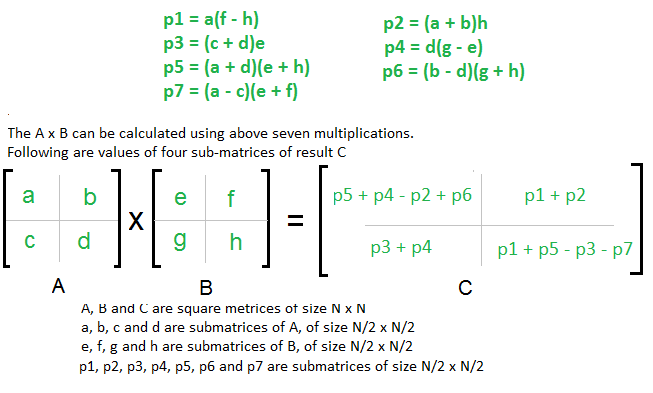
\includegraphics[scale=0.7]{strassen.png}
    \caption{Strassen's Method}
    \caption*{Source: www.geeksforgeeks.com}
\end{figure}

\begin{equation*}
    T(n) = 7T(\frac{n}{2}) + O(n^2)
\end{equation*}

We can use the Master's Theorem to compute the time complexity of Strassen's algorithm. We have 7 recursive calls and all the additions and subtractions take $O(n^2)$ time. Therefore the total time complexity turns out to be $O(n^{log 7})$.






\section{Empirical Comparison}
\subsection{System Specifications}
\textbf{Processor:} Intel Core i5 8250U\\
\textbf{RAM:} 12 GB\\
\textbf{Power Saving:} Max Performance Mode\\
\textbf{Language:} Python 3.8.1\\
\subsection{Data}
\begin{tabular}{|c|c|c|c|c|c|}
    \hline
     & & \multicolumn{4}{c|}{\textbf{Dimensions }($n \times n$)}\\
    \cline{3-6}
     & & \textbf{1024} & \textbf{512} & \textbf{256} & \textbf{128}  \\
     \hline
    \multirow{2}{*}{\textbf{Avg. Run-time (s)}} & \textbf{Naive Method} & 2207 & 286 & 32 & 5 \\
    \cline{2-6}
     & \textbf{Strassen's Method} & 3211 & 496 & 64 & 8.7 \\
    \hline
\end{tabular}

\begin{figure}[h!]
    \centering
    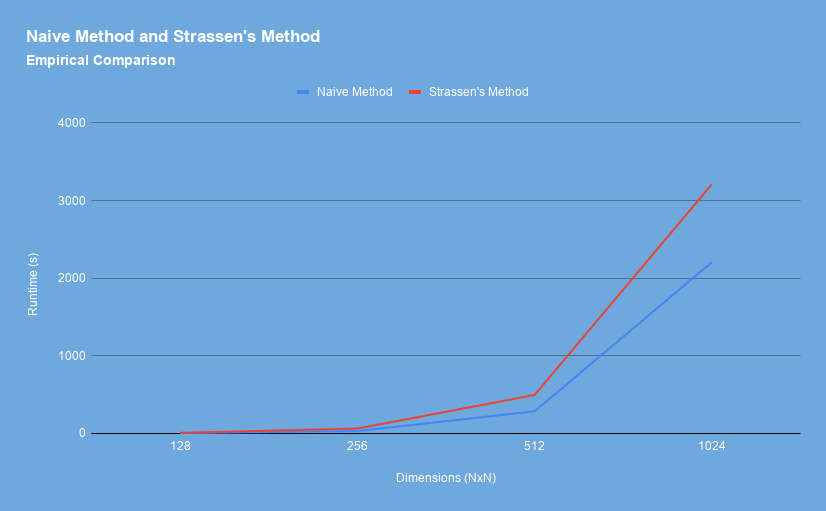
\includegraphics[scale=0.4]{chart.png}
    \caption{Empirical Comparison between Naive Method \& Strassen's Method}
\end{figure}


\subsection{Why Strassen's Method took longer?}
As can be noted from the aforementioned table Strassen's empirical analysis shows that it takes longer than the naive method regardless of the size of the matrix n. This is the result of communication bottlenecks that happen in real-time. These bottle necks arise due to the fact that a single call to the function implies that recursively the function will be called again and these recursive calls are waiting for each subsequent calls to reach the base case causing a lag.

\section{Feedback}
\begin{itemize}
    \item C++ should've been chosen as a language since it is faster than Python
\end{itemize}

\section{Conclusion}
Matrix multiplication is a very important aspect of Computer Science since it allows faster and more efficient mathematical modelling of real-world phenomena. There are other algorithms that do exist for this purpose but are beyond the goal of this project.

\end{document}
